\section{Auswertung}
\label{sec:Auswertung}
\subsection{Eichung der Zeitskala des Diskriminators}
Ein Plot der aufgenommenen Daten zur Eichung der Zeitachse mittels des Doppelpulsgenerators ist in \autoref{fig:zeit_fit} zu finden. Dort ist die Pulsbreite gegen die Kanalnummer aufgetragen. Durch die Kenntnis der gleichmäßigen Pulsabstände lässt sich die Zeitskala der Kanäle eichen, denn der Kanal, in welchem der zweite Puls des Doppelpulsgenerators gemessen wurde gibt an, wie viele Zeiteinheiten bis zur Messung des Pulses vergangen sind. Da die Relation zwischen Pulsbreite und Kanalnummer linear ist 
\begin{aquation}
    T_\text{Puls}(N_\text{Kanal}) &= T N_\text{Kanal} + T_0 \tp
\end{aquation}
Dabei hat die Zeitkonstante $\tau$ die Einheit $\text{Zeit}/\text{Kanal}$ und ist die Dauer, die ein Event in einem Kanal bedient wird, bevor der Detektor zum Nächsten springt.\\
Durch den linearen Fit, welcher zusätzlich in \autoref{fig:zeit_fit} abgebildet ist, wurde $T = (21,66 \pm 0,02)\text{ns}$ bestimmt.
\begin{figure}
    \centering
    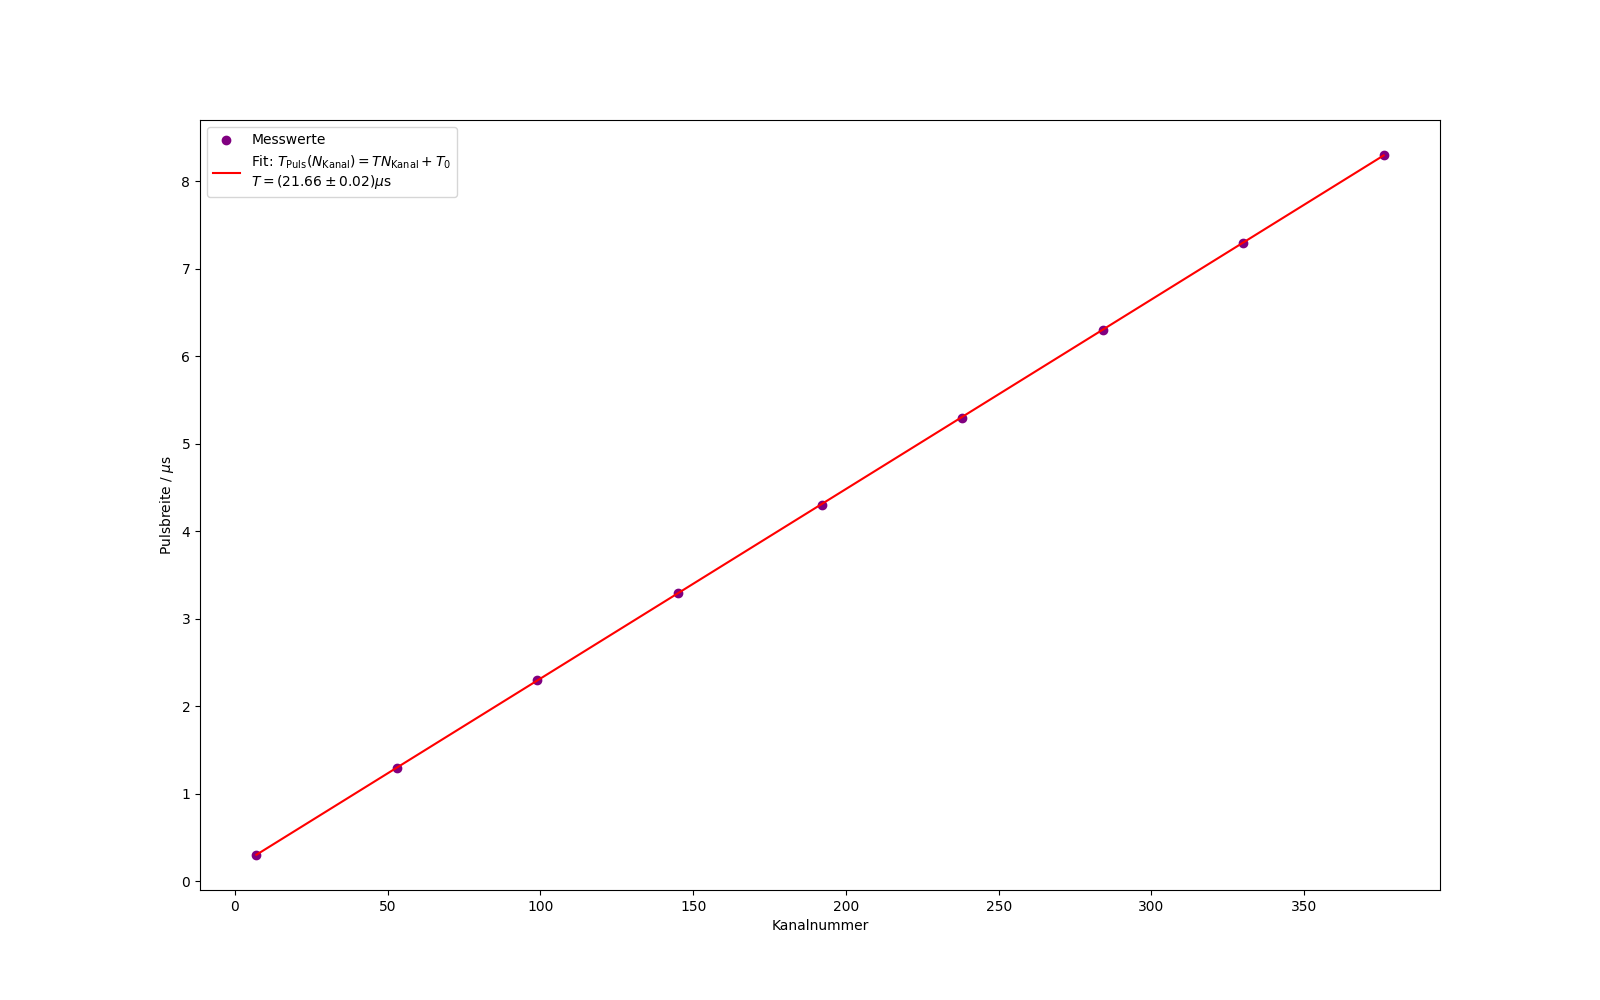
\includegraphics[width=\linewidth]{figures/time_fit.png}
    \caption{Linearer Fit zur Eichung des Diskriminators. Die Steigung der Geraden, $T = (21,66 \pm 0,02)\text{ns}$ ist die errechnete Zeit pro Kanal.}
    \label{fig:zeit_fit}
\end{figure}


\subsection{Bestimmung der mittleren Lebensdauer kosmischer Myonen}
Da die Spannung am Detektor zu hoch eingestellt war, sind die aufgenommenen Daten an ihrem Anfang durch eine Spannungsspitze überlagert und daher nicht verwendbar. Aus diesem Grund wurden hier die ersten $30$ Kanäle nicht verwendet. Außerdem wurden die letzten $150$ aufgenommenen Datenpunkte ebenfalls nicht verwendet, da dort quasi kein Signal mehr gemessen wurde.\\
Zur Bestimmung der Cutoffs wurden verschiedene Cutoffs getestet und jeweils ein Fit durchgeführt. Dabei wurde überprüft, wie das Entfernen weiterer Datenpunkte die Lebenszeit beeinflusst, um ein Gebiet zu erreichen, in welchem sich bei $\pm 10$ Datenpunkten kaum noch etwas an der bestimmten Lebenszeit der kosmischen Myonen ändert.\\
Die Standardabweichung einer Poissonverteilten Zufallsvariable wie den Counts ist $ \sigma = \sqrt{N}$. Diese ist in \autoref{fig:halflife} als Fehlerbalken der einzelnen Messwerte aufgetragen.\\
Um die Lebenszeit der kosmischen Müons zu bestimmen, wurden die Daten mit der Exponentialfunktion 
\begin{aquation}
    N\left(t\right) &= N_0 \exp\left(-\frac{t}{\tau}\right)
\end{aquation}
gefittet.\\
Als mittlere Lebensdauer ergibt sich aus dem Fit $\tau = (2,07 \pm 0,09)\text{$\mu$s}$.


\begin{figure}
    \centering
    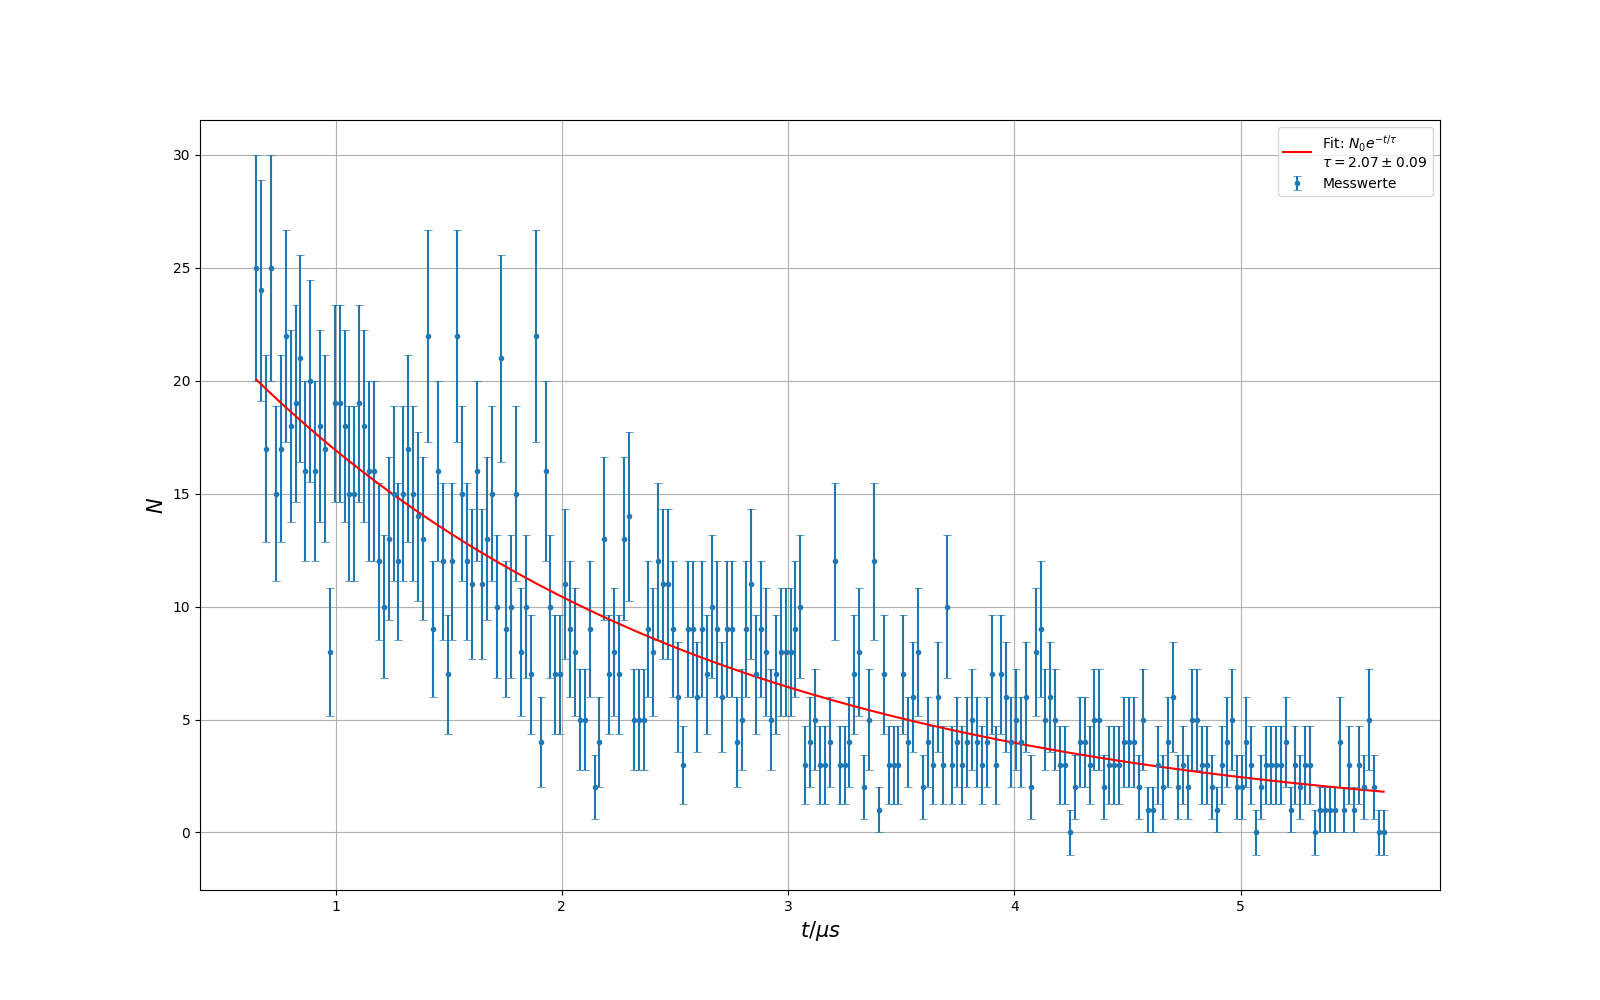
\includegraphics[width=\linewidth]{figures/halflife_fit.png}
    \caption{Fit zur Bestimmung der Halbwertszeit kosmischer Myonen.}
    \label{fig:halflife}
\end{figure}


